\documentclass[tikz,border=7pt]{standalone}
\begin{document}
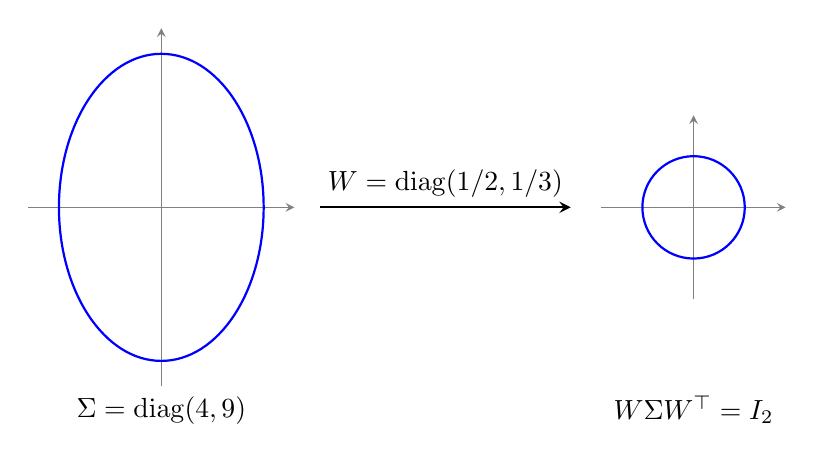
\begin{tikzpicture}[scale=.65,>=stealth]
\draw[->,gray] (-2.6,0)--(2.6,0);
\draw[->,gray] (0,-3.5)--(0,3.5);
\draw[blue,thick] (0,0) ellipse (2 and 3);
\node[below] at (0,-3.5) {$\Sigma=\mathrm{diag}(4,9)$};
\draw[->,thick] (3.1,0)--node[above] {$W=\mathrm{diag}(1/2,1/3)$} (8,0);
\draw[->,gray] (8.6,0)--(12.2,0);
\draw[->,gray] (10.4,-1.8)--(10.4,1.8);
\draw[blue,thick] (10.4,0) circle (1);
\node[below] at (10.4,-3.5) {$W\Sigma W^\top=I_2$};
\end{tikzpicture}
\end{document}
